\begin{figure}[htbp]
\begin{subfigure}{.48\textwidth}
\includegraphics[width=\textwidth]{images/results/pt-nofs-acc.eps}
\caption{}
\label{}
\end{subfigure}%
\begin{subfigure}{.55\textwidth}
\includegraphics[width=\textwidth]{images/results/pt-nofs-auc.eps}
\caption{}
\label{}
\end{subfigure}

\begin{subfigure}{.48\textwidth}
\includegraphics[width=\textwidth]{images/results/pt-cfs-acc.eps}
\caption{}
\label{}
\end{subfigure}%
\begin{subfigure}{.55\textwidth}
\includegraphics[width=\textwidth]{images/results/pt-cfs-auc.eps}
\caption{}
\label{}
\end{subfigure}

\begin{subfigure}{.48\textwidth}
\includegraphics[width=\textwidth]{images/results/pt-wrapper-acc.eps}
\caption{}
\label{}
\end{subfigure}%
\begin{subfigure}{.55\textwidth}
\includegraphics[width=\textwidth]{images/results/pt-wrapper-auc.eps}
\caption{}
\label{}
\end{subfigure}
\caption{Comparison of accuracy and AUC between classifiers for each non-threshold feature selection method, grouped by whether or not discretisation was applied.}
\label{fig:pt-nothreshold}
\end{figure}

\begin{figure}[htbp]
\begin{subfigure}{\textwidth}
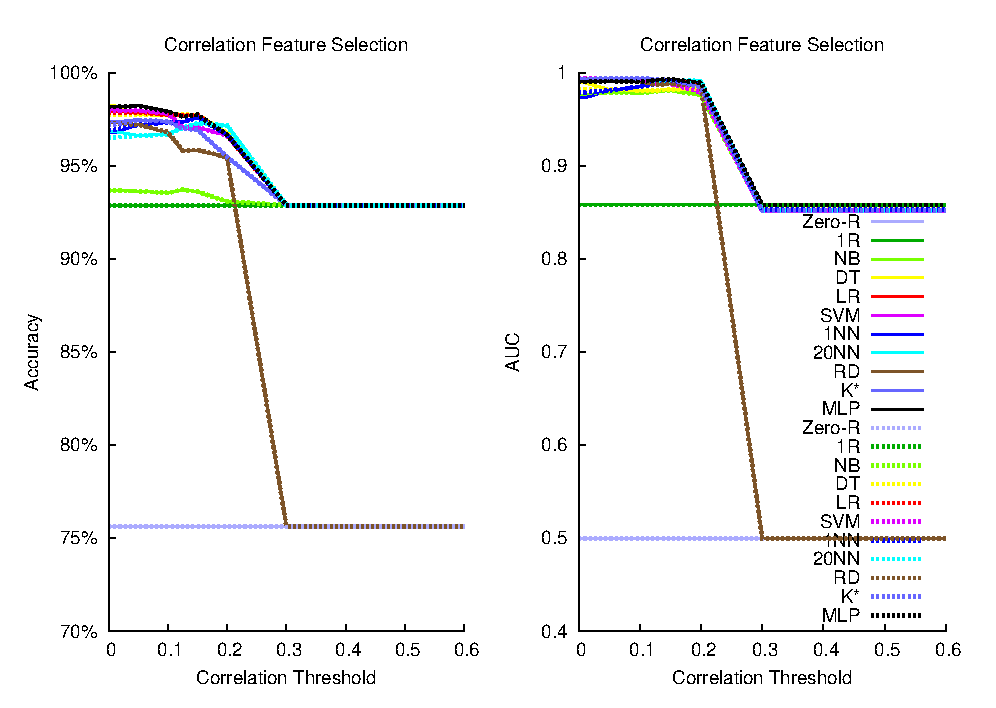
\includegraphics[width=\textwidth]{images/results/pt-corr.eps}
\caption{}
\label{fig:pt-threshold-corr}
\end{subfigure}
\ContinuedFloat
\begin{subfigure}{\textwidth}
\includegraphics[width=\textwidth]{images/results/pt-ig.eps}
\caption{}
\label{}
\end{subfigure}
\caption{Comparison of accuracy and AUC between classifiers for feature selectors that discard features based on a threshold. Solid lines correspond to a result without discretisation, and dashed lines correspond to a result with discretisation.}
\label{fig:pt-threshold}
\end{figure}

\begin{figure}[htbp]
\ContinuedFloat
\begin{subfigure}{\textwidth}
\includegraphics[width=\textwidth]{images/results/pt-oner.eps}
\caption{}
\label{}
\end{subfigure}
\caption[]{Comparison of accuracy and AUC between classifiers for feature selectors that discard features based on a threshold. Solid lines correspond to a result without discretisation, and dashed lines correspond to a result with discretisation.}
\end{figure}

